\documentclass[a4paper,11pt]{article}

\input ../include/preamble.tex

\usepackage{pgf-umlsd}
\usepgflibrary{arrows} % for pgf-umlsd
\usetikzlibrary{fit, positioning}

\begin{document}


\title{Pong - the first console game}

\author{Johan Montelius}
\date{Spring Term 2023}

\maketitle

\defaultpagestyle

\section*{Introduction}

This is an exercise in building an interactive game with two players
coordinated by one Elixir game engine. We will build the application
as a set of communicating processes where some processes are handling
the lower communication layers, one process is responsible for the
game logic and one to supervise and coordinate the actions. We will
use a web interface to handle the graphical dsiplay and forward input
from the players so there is some limited HTML and JS programing
involved.

The true reasoin why you want to do this exercise is of course that
the Pong game was a epiq game, one of the first console games, that
changed the world for ever. 

\section*{The game of Pong}

The game of Pong is a very simple model of a game of tennis. The two
opponents can only move their paddle up and down along the base line
and the bal will bounce of the walls on the upper and lower side
walls. If a player fails to return the ball by having the paddle in
the right position she looses a point and the opponent gets to serve a
new ball.

A ball will bounce of the side walls in a perfect reflection but the
bounce from a paddle is slightly off depending on how far from the
center of the paddle that ball hits i.e. not the movement of the
paddle. This behaviour will simulate spinning the ball and allows you
make a tougher return for the opponent to catch. 

\begin{figure}[t]
  \center 
  \includegraphics[scale=0.1]{pong.png}

  \caption{The game of Pong}
  \label{fig:pong}
\end{figure}

The classical Atari Game of Pong was played using a small console
attached to a TV. In our implementation we will of course use the
Internet and allow the two players to be anywhere as long as they have
a network connection. The look and feel should however be as in the orignal version shown in Fig.~\ref{fig:pong}.

\section*{The architecture}
  
When we implement this game it is a lot easier to first divide the
system into processes that handle various aspects of the game. The
system will consist of: a client part, processes on the server side
that handles the communication with each player, a server process that
starts the game and keeps the game state and a module that describes
the rules of the game. The architecture is outlined in Fig.~\ref{fig:arch}. 

\subsection*{the client}

The client processes (browser 1 and 2 in Fig.~\ref{fig:arch}) will be
web browser that are responsible for displaying the game and forward
user interaction. The client beahviour is implemented in JavaScript
and found in {\tt pong.js}. Since this is not a course in web design
we will keep it as simple as possible and I don't think we could do it
any simpler.

The communication between the clients and
the server will be solved using something called {\em web
  sockets}. This is a bidirectional message protocol that is
iniatiated through a HTTP request. On the client side this will be
handled by teh JavaScript WebSocket library but on the server side we
will have to implement everything from scratch (or use the version you
will find in the git repo).

\subsection*{the server}

The heart of the system is the {\tt server} process. It is the process
that we first start and it is responsible for handling the game
state. To make the communication with the clients easier we add two
layers between the server and the clients. The low level details of
decoding and encoding websocket messages is handled by a {\tt handler}
process. It wil deliver messages as byte sequences to a {\tt session}
process that will translate the byte sequnces to more comprehendible
mesages that are delivered to the server. The session process will
also encode messages from teh server to byte sequences before sending
them to the handler process. 


\begin{figure}
  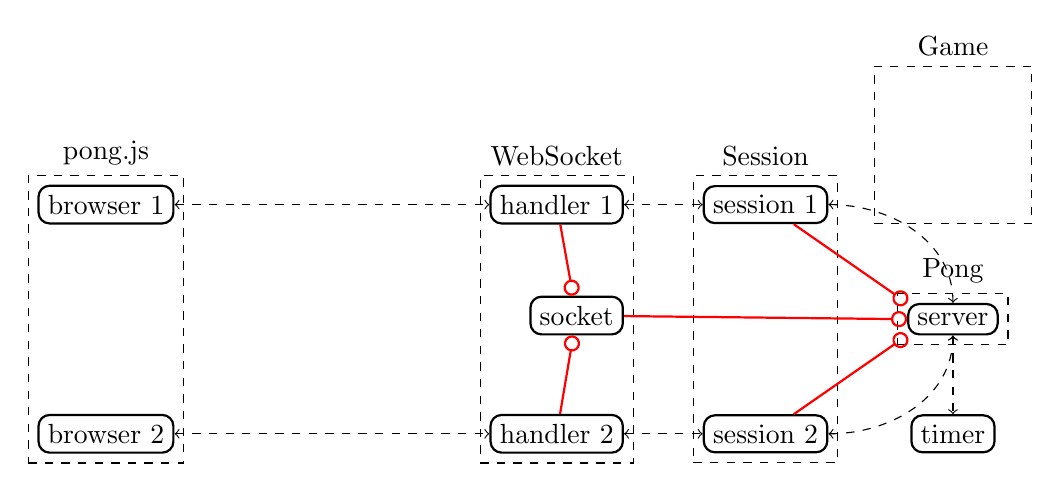
\begin{tikzpicture}[scale=0.5]
    \node[draw, thick, rounded corners] (server) at (0,0) {server};
    \node[draw, thick, rounded corners, above left = of server] (ses1) {session 1};
    \node[draw, thick, rounded corners, below left = of server] (ses2) {session 2};
    \node[draw, thick, rounded corners, below left = of ses1, above left = of ses2] (socket) {socket};
    \node[draw, thick, rounded corners, left = of ses1] (hdlr1) {handler 1};
    \node[draw, thick, rounded corners, left = of ses2] (hdlr2) {handler 2};
    \node[draw, thick, rounded corners, left = 4.0 cm of hdlr1] (brw1) {browser 1};
    \node[draw, thick, rounded corners, left = 4.0 cm of hdlr2] (brw2) {browser 2};
    \node[draw, thick, rounded corners, below = of server] (tmr) {timer};    

    \node[draw, dashed, fit = (server), label=Pong] {};
    \node[draw, dashed, fit = (ses1)(ses2), label=Session] {};
    \node[draw, dashed, fit = (socket)(hdlr1)(hdlr2), label=WebSocket] {};
    \node[draw, dashed, fit = (brw1)(brw2), label=pong.js] {};

    \node[draw, dashed, rectangle, label=Game, above = of server, minimum size=2cm] {};
    
    \draw[o-,thick, red] (server.west) -- (socket);
    \draw[o-,thick, red] (socket) -- (hdlr1);
    \draw[o-,thick, red] (socket) -- (hdlr2);
    \draw[o-,thick, red] (server.north west) -- (ses1);
    \draw[o-,thick, red] (server.south west) -- (ses2);            

    \draw[<->,dashed, black] (brw1) -- (hdlr1);
    \draw[<->,dashed, black] (brw2) -- (hdlr2);                    

    \draw[<->,dashed, black] (hdlr1) -- (ses1);    
    \draw[<->,dashed, black] (hdlr2) -- (ses2);

    \draw[<->,dashed, black] (ses1.east) to [out=0,in=90] (server.north);
    \draw[<->,dashed, black] (ses2.east) to [out=0,in=270] (server.south);
    \draw[<->,dashed, black] (server.south) to [out=270,in=90] (tmr.north);            
  \end{tikzpicture}
  \caption{The Pong architecture.}
  \label{fig:arch}
\end{figure}

The server process holds the state of the game and acts on either
client messages or clock ticks (wich will move the ball forward) but
it does not know much about how the game actually work. The game logic
is all defined in a module called {\tt Game}. This is where we decide
what to do if a user wants to move up or down or what happens if the
ball has moved. The Game module will know everything aboy how large
the court is, how balls bounce etc, it's much easier to keep all of
the details in one module.

\subsection*{the websocket layer}

The server will start by creating two processes, one {\tt server}
process for each player. It will then creat a {\tt socket} process
that is given the process identifiers of the two session
processes. The socket process will open a TCP listening socket on a
specified port and then spawn two processes that wait for incomming
connections.

To describe how the websocket protocol works in detail is a bit ouside
the scope of this exercise so let's only go through it breifly. A
client will open a connection by opening a TCP connection and then
send special HTTP request. This request will specify that it wants to
communicate over the websocket protocol so the server responds and
then keeps the connection open.

The clinent and the server can then communicate by sending encoded
message. The body of a message is a byte sequence so it up to us to
come up with a encoding of our messages as a byte sequence.

In order to handle the incoming messages the handler process will
spawn a decoder process that will listen and decode messages comming
from the client. Some low level socket messages it can reply to itself
but when it has received a proper message it will send it to the
handler process.

The handler process will receive messages from the decoder process and
forward them to its session process. The 









\end{document}
